\documentclass[tikz,border=15pt]{standalone}
\usepackage{tikz}
\usepackage{amsmath,amssymb}
\usetikzlibrary{arrows.meta,positioning,shapes.geometric,shapes.misc,fit,backgrounds,calc,shadows}

% ==============================================================================
% Color Palette Definitions (High-contrast academic hardware architecture style)
% ==============================================================================
\definecolor{primaryA}{HTML}{0284C7}     % Cyan/Blue (Region A - WS)
\definecolor{primaryAbg}{HTML}{E0F2FE}   % Light Sky Blue
\definecolor{primaryAdark}{HTML}{0369A1} % Deep Blue

\definecolor{primaryB}{HTML}{D97706}     % Amber/Orange (Region B - OS)
\definecolor{primaryBbg}{HTML}{FEF3C7}   % Light Amber
\definecolor{primaryBdark}{HTML}{B45309} % Deep Amber

\definecolor{barrierCol}{HTML}{DC2626}   % Red (Dynamic Boundary Barrier)
\definecolor{barrierBg}{HTML}{FEE2E2}    % Soft Red
\definecolor{barrierDark}{HTML}{991B1B}  % Deep Red

\definecolor{memCol}{HTML}{4F46E5}       % Indigo (Memory Substrate)
\definecolor{memBg}{HTML}{EEF2FF}        % Light Indigo
\definecolor{memDark}{HTML}{312E81}      % Dark Indigo

\definecolor{ctrlCol}{HTML}{7C3AED}      % Purple (Controllers & Arbiters)
\definecolor{ctrlBg}{HTML}{F5F3FF}       % Light Purple
\definecolor{ctrlDark}{HTML}{4C1D95}     % Dark Purple

\definecolor{secCol}{HTML}{BE123C}       % Rose/Maroon (Scrub & Security)
\definecolor{secBg}{HTML}{FFE4E6}        % Light Rose

\definecolor{panelBg}{HTML}{F8FAFC}      % Neutral Slate White
\definecolor{cardBorder}{HTML}{94A3B8}   % Slate Border
\definecolor{textDark}{HTML}{0F172A}     % Dark Navy Text

\begin{document}
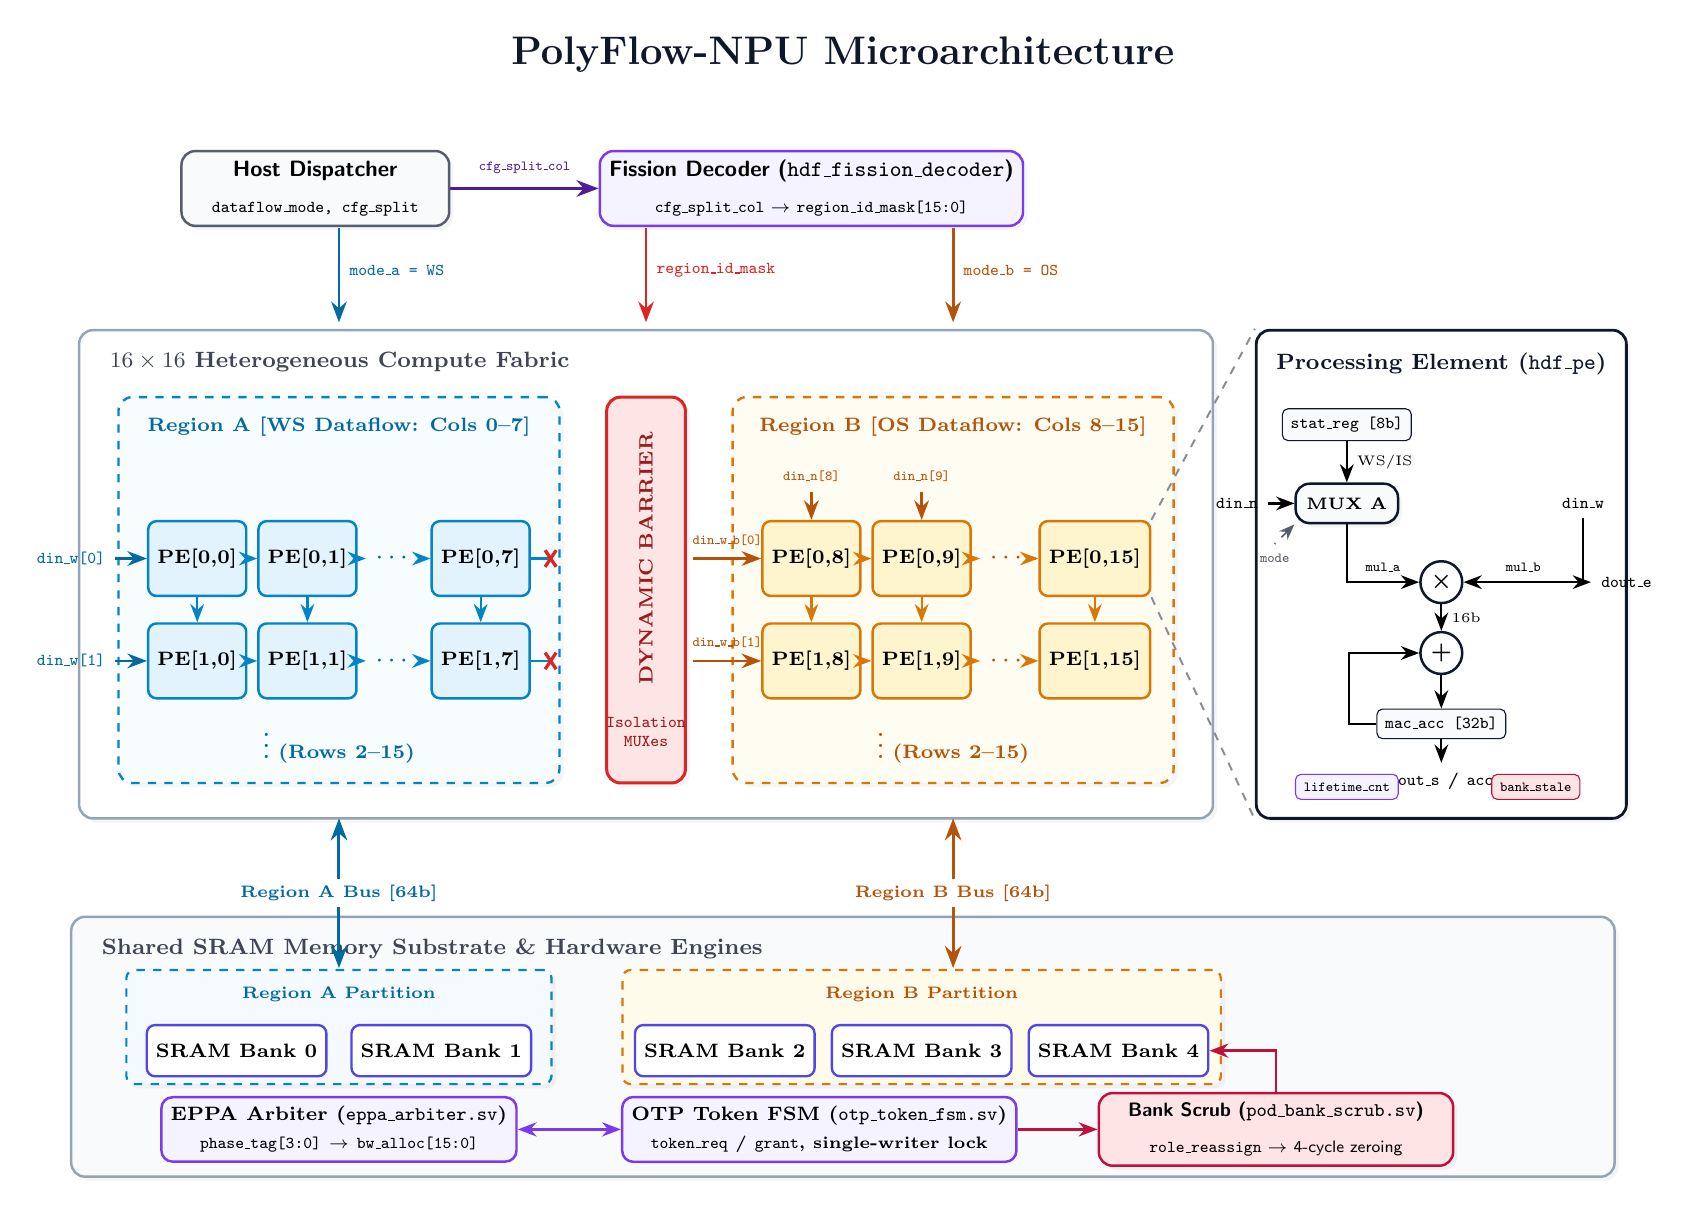
\begin{tikzpicture}[
    font=\sffamily,
    >=Stealth,
    every node/.style={align=center},
    card/.style={
        draw=cardBorder,
        fill=white,
        rounded corners=5pt,
        line width=0.9pt,
        drop shadow={opacity=0.08, shadow xshift=1.5pt, shadow yshift=-1.5pt}
    },
    peA/.style={
        draw=primaryA,
        fill=primaryAbg!90,
        rounded corners=3pt,
        line width=0.9pt,
        minimum width=1.15cm,
        minimum height=0.95cm,
        font=\fontsize{7.5}{9}\selectfont\bfseries
    },
    peB/.style={
        draw=primaryB,
        fill=primaryBbg!90,
        rounded corners=3pt,
        line width=0.9pt,
        minimum width=1.15cm,
        minimum height=0.95cm,
        font=\fontsize{7.5}{9}\selectfont\bfseries
    },
    bankNode/.style={
        draw=memCol,
        fill=white,
        rounded corners=3pt,
        line width=0.85pt,
        minimum width=1.95cm,
        minimum height=0.65cm,
        font=\fontsize{7.5}{8.5}\selectfont\bfseries
    },
    ctrlNode/.style={
        draw=ctrlCol,
        fill=ctrlBg,
        rounded corners=4pt,
        line width=0.9pt,
        minimum width=4.4cm,
        minimum height=0.75cm,
        font=\fontsize{7.5}{9}\selectfont\bfseries
    },
    mathNode/.style={
        draw=textDark,
        fill=white,
        circle,
        inner sep=1.8pt,
        line width=0.9pt,
        font=\fontsize{8}{9}\selectfont\bfseries
    },
    regNode/.style={
        draw=textDark,
        fill=panelBg,
        rounded corners=2pt,
        inner sep=3pt,
        font=\fontsize{6.5}{7.5}\selectfont\bfseries
    }
]

  % ============================================================================
  % TITLE
  % ============================================================================
  \node[font=\fontsize{14}{17}\selectfont\bfseries\color{textDark}] (title) at (10.0, 14.3) 
      {PolyFlow-NPU Microarchitecture};

  % ============================================================================
  % 1. TOP CONTROL LAYER (Host Dispatcher & Fission Decoder)
  % ============================================================================
  \node[card, draw=textDark!70, fill=panelBg, minimum width=3.4cm, minimum height=0.95cm] (host_sched) at (3.3, 12.6) {
      \textbf{\fontsize{8.5}{10}\selectfont Host Dispatcher}\\[1pt]
      \fontsize{6.5}{7.5}\selectfont\texttt{dataflow\_mode, cfg\_split}
  };

  \node[card, draw=ctrlCol, fill=ctrlBg, minimum width=4.6cm, minimum height=0.95cm] (fiss_dec) at (9.6, 12.6) {
      \textbf{\fontsize{8.5}{10}\selectfont Fission Decoder (\texttt{hdf\_fission\_decoder})}\\[1pt]
      \fontsize{6.5}{7.5}\selectfont\texttt{cfg\_split\_col} $\to$ \texttt{region\_id\_mask[15:0]}
  };

  % Connecting Bus between Dispatcher and Decoder
  \draw[->, line width=1.1pt, color=ctrlDark] (host_sched.east) -- (fiss_dec.west)
      node[midway, above=1.5pt, font=\fontsize{5.5}{6.5}\selectfont\bfseries] {\texttt{cfg\_split\_col}};

  % 3 Straight Vertical Control Buses (Strictly Symmetric, Zero Crossings)
  \draw[->, line width=1.0pt, color=primaryAdark] (3.6, 12.1) -- (3.6, 10.9)
      node[pos=0.45, right, font=\fontsize{6.5}{7.5}\selectfont\bfseries\color{primaryAdark}] {\texttt{mode\_a = WS}};

  \draw[->, line width=1.0pt, color=barrierCol] (7.5, 12.1) -- (7.5, 10.9)
      node[pos=0.45, right, font=\fontsize{6.5}{7.5}\selectfont\bfseries\color{barrierDark}] {\texttt{region\_id\_mask}};

  \draw[->, line width=1.0pt, color=primaryBdark] (11.4, 12.1) -- (11.4, 10.9)
      node[pos=0.45, right, font=\fontsize{6.5}{7.5}\selectfont\bfseries\color{primaryBdark}] {\texttt{mode\_b = OS}};

  % ============================================================================
  % 2. 2D COMPUTE FABRIC (Center Left)
  % ============================================================================
  \node[card, fill=white, minimum width=14.4cm, minimum height=6.2cm] (array_box) at (7.5, 7.7) {};
  \node[anchor=north west, font=\fontsize{8}{9}\selectfont\bfseries\color{textDark!80}] at ([xshift=8pt, yshift=-5pt]array_box.north west) 
      {$16 \times 16$ Heterogeneous Compute Fabric};

  % ----------------------------------------------------------------------------
  % Region A Sub-Array (Cols 0-7)
  % ----------------------------------------------------------------------------
  \node[card, draw=primaryA, fill=primaryAbg!25, dashed, line width=0.85pt, minimum width=5.6cm, minimum height=4.9cm] (regA) at (3.6, 7.5) {};
  \node[anchor=north, font=\fontsize{7.5}{8.5}\selectfont\bfseries\color{primaryAdark}] at ([yshift=-4pt]regA.north) 
      {Region A [WS Dataflow: Cols 0--7]};

  % Region A PE Nodes
  \node[peA] (pe00) at (1.8, 7.9) {PE[0,0]};
  \node[peA] (pe01) at (3.2, 7.9) {PE[0,1]};
  \node[font=\bfseries\color{primaryAdark}] (pe0dots) at (4.3, 7.9) {$\cdots$};
  \node[peA] (pe07) at (5.4, 7.9) {PE[0,7]};

  \node[peA] (pe10) at (1.8, 6.6) {PE[1,0]};
  \node[peA] (pe11) at (3.2, 6.6) {PE[1,1]};
  \node[font=\bfseries\color{primaryAdark}] (pe1dots) at (4.3, 6.6) {$\cdots$};
  \node[peA] (pe17) at (5.4, 6.6) {PE[1,7]};

  \node[font=\fontsize{7.5}{9}\selectfont\bfseries\color{primaryAdark}] at (3.6, 5.6) {$\vdots$ (Rows 2--15)};

  % Region A Mesh Arrows
  \draw[->, line width=0.8pt, color=primaryA] (pe00) -- (pe01);
  \draw[->, line width=0.8pt, color=primaryA] (pe01) -- (pe0dots);
  \draw[->, line width=0.8pt, color=primaryA] (pe0dots) -- (pe07);

  \draw[->, line width=0.8pt, color=primaryA] (pe10) -- (pe11);
  \draw[->, line width=0.8pt, color=primaryA] (pe11) -- (pe1dots);
  \draw[->, line width=0.8pt, color=primaryA] (pe1dots) -- (pe17);

  \draw[->, line width=0.8pt, color=primaryA] (pe00) -- (pe10);
  \draw[->, line width=0.8pt, color=primaryA] (pe01) -- (pe11);
  \draw[->, line width=0.8pt, color=primaryA] (pe07) -- (pe17);

  % Region A Inputs
  \draw[<-, line width=0.9pt, color=primaryAdark] (pe00.west) -- ++(-0.4,0) 
      node[left, font=\fontsize{6}{7}\selectfont\bfseries] {\texttt{din\_w[0]}};
  \draw[<-, line width=0.9pt, color=primaryAdark] (pe10.west) -- ++(-0.4,0) 
      node[left, font=\fontsize{6}{7}\selectfont\bfseries] {\texttt{din\_w[1]}};

  % ----------------------------------------------------------------------------
  % Dynamic Boundary Barrier
  % ----------------------------------------------------------------------------
  \node[card, draw=barrierCol, fill=barrierBg!90, line width=1.1pt, minimum width=1.0cm, minimum height=4.9cm] (barrier) at (7.5, 7.5) {};
  \node[rotate=90, font=\fontsize{7.5}{8.5}\selectfont\bfseries\color{barrierDark}] at (7.5, 7.9) 
      {DYNAMIC BARRIER};
  \node[font=\fontsize{6}{7}\selectfont\bfseries\color{barrierDark}] at (7.5, 5.7) 
      {\texttt{Isolation}\\\texttt{MUXes}};

  % Barrier Cuts (Visual Isolation Markers)
  \draw[line width=0.8pt, color=primaryA] (pe07.east) -- ++(0.25,0) coordinate (cut0);
  \draw[line width=1.2pt, color=barrierCol] ([xshift=-2pt, yshift=-3pt]cut0) -- ([xshift=2pt, yshift=3pt]cut0);
  \draw[line width=1.2pt, color=barrierCol] ([xshift=-2pt, yshift=3pt]cut0) -- ([xshift=2pt, yshift=-3pt]cut0);

  \draw[line width=0.8pt, color=primaryA] (pe17.east) -- ++(0.25,0) coordinate (cut1);
  \draw[line width=1.2pt, color=barrierCol] ([xshift=-2pt, yshift=-3pt]cut1) -- ([xshift=2pt, yshift=3pt]cut1);
  \draw[line width=1.2pt, color=barrierCol] ([xshift=-2pt, yshift=3pt]cut1) -- ([xshift=2pt, yshift=-3pt]cut1);

  % ----------------------------------------------------------------------------
  % Region B Sub-Array (Cols 8-15)
  % ----------------------------------------------------------------------------
  \node[card, draw=primaryB, fill=primaryBbg!25, dashed, line width=0.85pt, minimum width=5.6cm, minimum height=4.9cm] (regB) at (11.4, 7.5) {};
  \node[anchor=north, font=\fontsize{7.5}{8.5}\selectfont\bfseries\color{primaryBdark}] at ([yshift=-4pt]regB.north) 
      {Region B [OS Dataflow: Cols 8--15]};

  % Region B PE Nodes
  \node[peB] (pe08) at (9.6, 7.9) {PE[0,8]};
  \node[peB] (pe09) at (11.0, 7.9) {PE[0,9]};
  \node[font=\bfseries\color{primaryBdark}] (pe0dotsB) at (12.1, 7.9) {$\cdots$};
  \node[peB] (pe015) at (13.2, 7.9) {PE[0,15]};

  \node[peB] (pe18) at (9.6, 6.6) {PE[1,8]};
  \node[peB] (pe19) at (11.0, 6.6) {PE[1,9]};
  \node[font=\bfseries\color{primaryBdark}] (pe1dotsB) at (12.1, 6.6) {$\cdots$};
  \node[peB] (pe115) at (13.2, 6.6) {PE[1,15]};

  \node[font=\fontsize{7.5}{9}\selectfont\bfseries\color{primaryBdark}] at (11.4, 5.6) {$\vdots$ (Rows 2--15)};

  % Region B Mesh Arrows
  \draw[->, line width=0.8pt, color=primaryB] (pe08) -- (pe09);
  \draw[->, line width=0.8pt, color=primaryB] (pe09) -- (pe0dotsB);
  \draw[->, line width=0.8pt, color=primaryB] (pe0dotsB) -- (pe015);

  \draw[->, line width=0.8pt, color=primaryB] (pe18) -- (pe19);
  \draw[->, line width=0.8pt, color=primaryB] (pe19) -- (pe1dotsB);
  \draw[->, line width=0.8pt, color=primaryB] (pe1dotsB) -- (pe115);

  \draw[->, line width=0.8pt, color=primaryB] (pe08) -- (pe18);
  \draw[->, line width=0.8pt, color=primaryB] (pe09) -- (pe19);
  \draw[->, line width=0.8pt, color=primaryB] (pe015) -- (pe115);

  % Region B Dedicated Inputs (Zero Collision)
  \draw[->, line width=0.9pt, color=primaryBdark] (8.1, 7.9) -- (pe08.west) 
      node[above=1pt, midway, font=\fontsize{5.5}{6.5}\selectfont\bfseries] {\texttt{din\_w\_b[0]}};
  \draw[->, line width=0.9pt, color=primaryBdark] (8.1, 6.6) -- (pe18.west) 
      node[above=1pt, midway, font=\fontsize{5.5}{6.5}\selectfont\bfseries] {\texttt{din\_w\_b[1]}};

  \draw[<-, line width=0.9pt, color=primaryBdark] (pe08.north) -- ++(0,0.35) 
      node[above, font=\fontsize{5.5}{6.5}\selectfont\bfseries] {\texttt{din\_n[8]}};
  \draw[<-, line width=0.9pt, color=primaryBdark] (pe09.north) -- ++(0,0.35) 
      node[above, font=\fontsize{5.5}{6.5}\selectfont\bfseries] {\texttt{din\_n[9]}};

  % ============================================================================
  % 3. PE MICROARCHITECTURE INSET (Right Side - Exact RTL Datapath)
  % ============================================================================
  \node[card, draw=textDark, fill=white, line width=1.0pt, minimum width=4.7cm, minimum height=6.2cm] (pe_schematic) at (17.6, 7.7) {};
  \node[anchor=north, font=\fontsize{8}{9}\selectfont\bfseries\color{textDark}] at ([yshift=-5pt]pe_schematic.north) 
      {Processing Element (\texttt{hdf\_pe})};

  % Preload / Stationary Register
  \node[regNode, minimum width=1.4cm] (stat_reg) at (16.4, 9.6) {\texttt{stat\_reg [8b]}};

  % MUX A (selects mul_a: stat_reg vs din_n)
  \node[card, draw=textDark, fill=panelBg, inner sep=2pt, minimum width=1.3cm, minimum height=0.5cm, font=\fontsize{6.5}{7.5}\selectfont\bfseries] (mux_a) at (16.4, 8.6) {MUX A};

  % Connections to MUX A
  \draw[->, line width=0.8pt] (stat_reg.south) -- node[right, font=\fontsize{5}{6}\selectfont] {WS/IS} (mux_a.north);
  \draw[->, line width=0.8pt] (15.4, 8.6) node[left, font=\fontsize{6}{7}\selectfont\bfseries] {\texttt{din\_n}} -- (mux_a.west);
  \draw[<-, line width=0.6pt, dashed, color=textDark!70] (mux_a.south west) -- ++(-0.25,-0.25)
      node[below, font=\fontsize{5}{6}\selectfont] {\texttt{mode}};

  % Direct din_w operand port
  \node[font=\fontsize{6}{7}\selectfont\bfseries] (in_w_pe) at (19.4, 8.6) {\texttt{din\_w}};

  % Multiplier
  \node[mathNode] (mul) at (17.6, 7.6) {$\boldsymbol{\times}$};
  \draw[->, line width=0.8pt] (mux_a.south) |- node[near end, above, font=\fontsize{5}{6}\selectfont] {\texttt{mul\_a}} (mul);
  \draw[->, line width=0.8pt] (in_w_pe.south) |- node[near end, above, font=\fontsize{5}{6}\selectfont] {\texttt{mul\_b}} (mul);

  % Adder & Accumulator
  \node[mathNode] (add) at (17.6, 6.7) {$\boldsymbol{+}$};
  \node[regNode, minimum width=1.4cm] (acc_reg) at (17.6, 5.8) {\texttt{mac\_acc [32b]}};
  \draw[->, line width=0.8pt] (mul) -- node[right, font=\fontsize{5}{6}\selectfont] {16b} (add);
  \draw[->, line width=0.8pt] (add) -- (acc_reg);
  \draw[->, line width=0.8pt] (acc_reg.west) -- ++(-0.35,0) |- (add);

  % Outputs (Systolic Pass-Through & Accumulator)
  \draw[->, line width=0.8pt] (acc_reg.south) -- ++(0,-0.3) 
      node[below, font=\fontsize{6}{7}\selectfont\bfseries] {\texttt{dout\_s} / \texttt{acc}};
  \draw[->, line width=0.8pt] (19.1, 7.6) -- ++(0.4,0) 
      node[right, font=\fontsize{6}{7}\selectfont\bfseries] {\texttt{dout\_e}};

  % Control Status Registers inside PE
  \node[regNode, draw=ctrlCol, fill=ctrlBg, font=\fontsize{5.5}{6.5}\selectfont] at (16.4, 5.0) {\texttt{lifetime\_cnt}};
  \node[regNode, draw=secCol, fill=secBg, font=\fontsize{5.5}{6.5}\selectfont] at (18.8, 5.0) {\texttt{bank\_stale}};

  % Callout Lines from PE[0,15]
  \draw[dashed, line width=0.7pt, color=textDark!50] (pe015.north east) -- (pe_schematic.north west);
  \draw[dashed, line width=0.7pt, color=textDark!50] (pe015.south east) -- (pe_schematic.south west);

  % ============================================================================
  % 4. MEMORY & ARBITRATION SUBSTRATE (Bottom Layer)
  % ============================================================================
  \node[card, fill=panelBg, minimum width=19.6cm, minimum height=3.3cm] (mem_box) at (10.0, 1.7) {};
  \node[anchor=north west, font=\fontsize{8}{9}\selectfont\bfseries\color{textDark!80}] at ([xshift=8pt, yshift=-5pt]mem_box.north west) 
      {Shared SRAM Memory Substrate \& Hardware Engines};

  % Inter-Layer Memory Buses (In open channel between cards, y = 3.65)
  \draw[<->, line width=1.1pt, color=primaryAdark] (3.6, 2.7) -- (3.6, 4.6)
      node[midway, fill=white, inner sep=2pt, font=\fontsize{6.5}{7.5}\selectfont\bfseries\color{primaryAdark}] 
      {Region A Bus [64b]};

  \draw[<->, line width=1.1pt, color=primaryBdark] (11.4, 2.7) -- (11.4, 4.6)
      node[midway, fill=white, inner sep=2pt, font=\fontsize{6.5}{7.5}\selectfont\bfseries\color{primaryBdark}] 
      {Region B Bus [64b]};

  % ----------------------------------------------------------------------------
  % Partition Group Boundaries (Labels Placed Inside Cards, Zero Collision)
  % ----------------------------------------------------------------------------
  % Region A SRAM Partition
  \node[card, draw=primaryA, dashed, fill=primaryAbg!35, rounded corners=3pt, line width=0.8pt, minimum width=5.4cm, minimum height=1.45cm] (grpA) at (3.6, 1.95) {};
  \node[anchor=north, font=\fontsize{6.5}{7.5}\selectfont\bfseries\color{primaryAdark}] at ([yshift=-3pt]grpA.north) 
      {Region A Partition};
  \node[bankNode] (bank0) at (2.3, 1.65) {SRAM Bank 0};
  \node[bankNode] (bank1) at (4.9, 1.65) {SRAM Bank 1};

  % Region B SRAM Partition
  \node[card, draw=primaryB, dashed, fill=primaryBbg!35, rounded corners=3pt, line width=0.8pt, minimum width=7.6cm, minimum height=1.45cm] (grpB) at (11.0, 1.95) {};
  \node[anchor=north, font=\fontsize{6.5}{7.5}\selectfont\bfseries\color{primaryBdark}] at ([yshift=-3pt]grpB.north) 
      {Region B Partition};
  \node[bankNode] (bank2) at (8.5, 1.65) {SRAM Bank 2};
  \node[bankNode] (bank3) at (11.0, 1.65) {SRAM Bank 3};
  \node[bankNode] (bank4) at (13.5, 1.65) {SRAM Bank 4};

  % ----------------------------------------------------------------------------
  % Hardware Management Controllers (Pure Architecture Blocks at y = 0.65)
  % ----------------------------------------------------------------------------
  \node[ctrlNode] (eppa_ctrl) at (3.6, 0.65) {
      \textbf{EPPA Arbiter (\texttt{eppa\_arbiter.sv})}\\[1pt]
      \fontsize{6}{7}\selectfont\texttt{phase\_tag[3:0]} $\to$ \texttt{bw\_alloc[15:0]}
  };

  \node[ctrlNode] (otp_ctrl) at (9.7, 0.65) {
      \textbf{OTP Token FSM (\texttt{otp\_token\_fsm.sv})}\\[1pt]
      \fontsize{6}{7}\selectfont\texttt{token\_req} / \texttt{grant}, single-writer lock
  };

  \node[card, draw=secCol, fill=secBg, minimum width=4.5cm, minimum height=0.75cm] (scrub_ctrl) at (15.5, 0.65) {
      \textbf{\fontsize{7.5}{9}\selectfont Bank Scrub (\texttt{pod\_bank\_scrub.sv})}\\[1pt]
      \fontsize{6}{7}\selectfont\texttt{role\_reassign} $\to$ 4-cycle zeroing
  };

  % Inter-Engine Handshakes
  \draw[<->, line width=0.85pt, color=ctrlCol] (eppa_ctrl) -- (otp_ctrl);
  \draw[->, line width=0.85pt, color=secCol] (otp_ctrl) -- (scrub_ctrl);
  \draw[->, line width=0.85pt, color=secCol] (scrub_ctrl.north) |- (bank4.east);

\end{tikzpicture}
\end{document}
